\subsection{Eksempel: Politisk analyse}
De fleste er kjent med den vanlige høyre-venstre-aksen som brukes til å visualisere politisk tilhørighet. Denne visualiseringen fungerer fordi det er stor sammenheng (kovarians) mellom mange av de viktigste sakene for de politiske partiene. De fleste av oss har antageligvis fordommer om at ulvemotstand gjerne fører med seg bompengemotstan, eller at veganisme henger sammen med motstand mot oljebransjen. Men stemmer disse antagelsene? NRK sin valgomat fra kommunevalget inneholder svar fra de ni partiene som er representert på stortinget om idelogiske spørsmål NRK sin journalister vurderte som de aller viktigste. Jeg antar at disse spørsmålene representerer partiene sine syn \textit{godt nok}. Ideelt sett skulle jeg hatt mer data, men disse 16 påstandene kan likevel si en del om hva slags akser politiske partier kan sorteres langs.

Partiene har på hver påstand svart ``Helt uenig'', ``Litt uenig'', ``Litt enig'' eller ``Helt enig''. Jeg har oversatt dette til poengscorer på hhv. $-2$, $-1$, $1$ og $2$, dvs. at ``Helt'' regnes som dobbelt så viktig som ``litt'' enig eller uenig. Denne vektingen kan også diskuteres, men en eller annen verdi må tross alt velges. Med denne dataen er det rett frem å bruke \textbf{The Unscrambler\texttrademark} til å gjennomføre en PCA, er egnet til å finne underliggende strukturer i multivariat data.

Resultatene av dette er vist i figur \ref{fig:politikk-pca}. EV-plottet viser at 80\% av variasjonen i dataen kan forklares med to politiske akser, men den kryssvaliderte dataen viser at et mer realistisk estimat er litt over 50\%. I en tid der mange er bekymret for polarisering, er det betryggende å se at norsk politikk ikke kan beskrives spesielt fullstendig langs kun én (eller to) akser.

Score-plottet viser at første PC mer eller mindre direkte representerer den vanlige høyre-venstre-aksen, men her også med egenskapen at den gir en absolutt verdi og ikke bare en rangering. Det er også artig å se at den er rotert $180^\circ$ sammenlignet med det vi er vant til å se, siden programvaren dessverre ikke klarer å plukke opp konvensjon for visuell formidling av politisk tilhørighet.

Den andre aksen er mindre tydelig, men ved å se på ytterpunktene kan det tenkes at den plukker opp en slags by-bygd-sammenheng (V og MdG sees typisk mer på som bypartier, mens Sp åpenbart går under kategorien bygd). Spesielt påstandene om EØS og ulv underbygger dette, der de befinner seg på motsatte sider langs denne aksen.

Score-plottet kan, med disse tolkningene definert, sees på som et politisk kompass av samme type som konservativ/liberal-liberterianer/autoritær som jeg har sett på internett før. Her vil imidlertid aksene være høyre/venstre-by/bygd. Kategoriseringen vil da være

\begin{itemize}
	\item \textbf{Venstre, by:} SV og MDG
	\item \textbf{Venstre, bygd:} Ap og R
	\item \textbf{Høyre, by:} V, H, KrF
	\item \textbf{Høyre, bygd:} FrP, SP
\end{itemize}
så kan man jo vurdere selv om dette stemmer med sine egne fordommer. Dette er kanskje ikke en grensesprengende analyse, men jeg synes likevel det er interessant å se at dataen underbygger det man ofte bare antar. I tillegg kan denne analysen, om man antar at utvalget av spørsmålet representerer det folk flest synes er viktig, si noe om hvor uenighetene er størst.

\begin{figure}[h]
 	\centering
 	\begin{subfigure}[t]{0.48\textwidth}
 		\centering
 		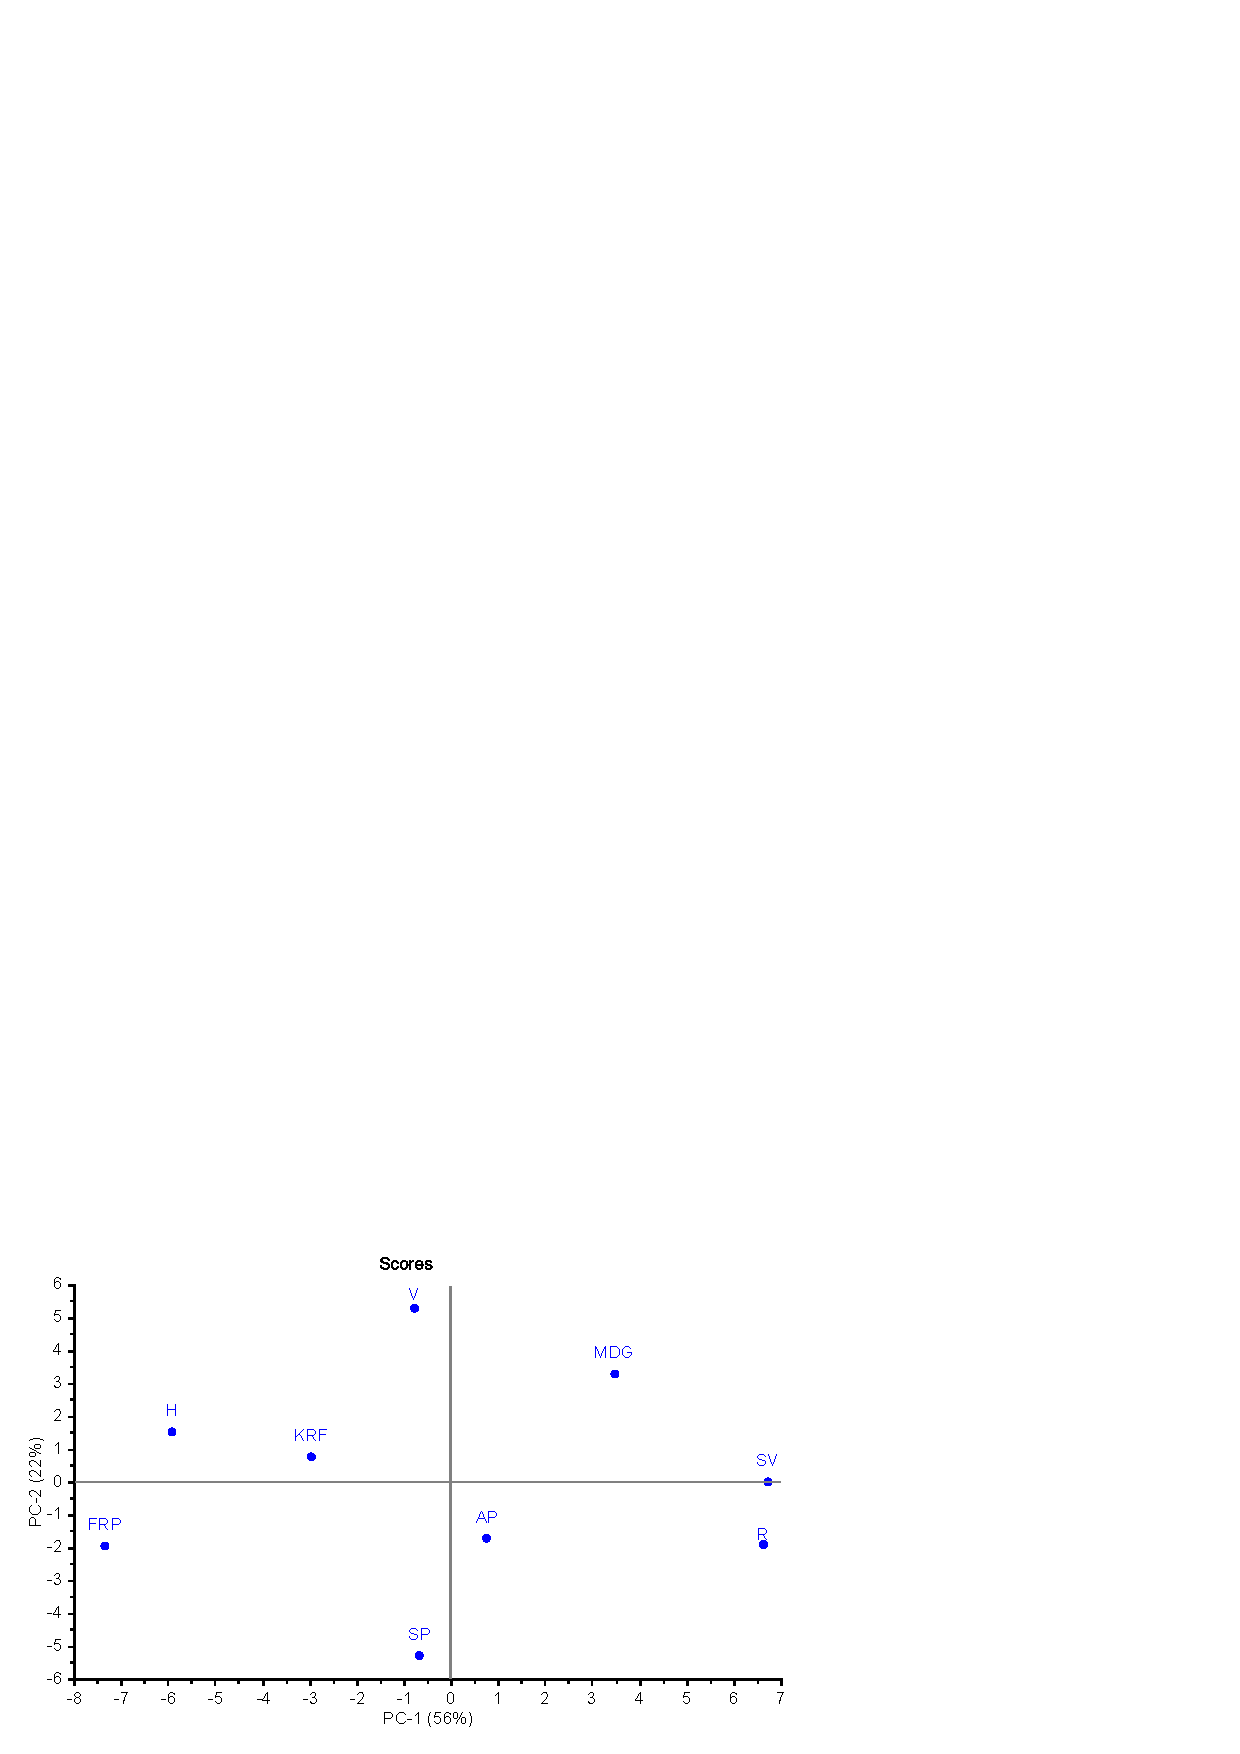
\includegraphics[width=\textwidth]{figurer/politikk-pca-scores}
 		\caption{}
 		\label{}
 	\end{subfigure}	
 	\begin{subfigure}[t]{0.48\textwidth}
 		\centering
 		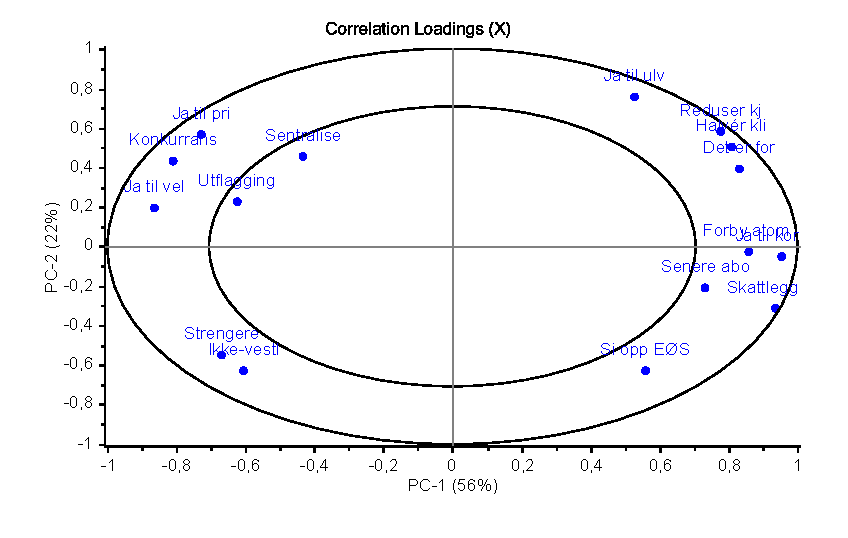
\includegraphics[width=\textwidth]{figurer/politikk-pca-loadings}
 		\caption{}
 		\label{}
 	\end{subfigure}
 	\begin{subfigure}[t]{0.48\textwidth}
 		\centering
 		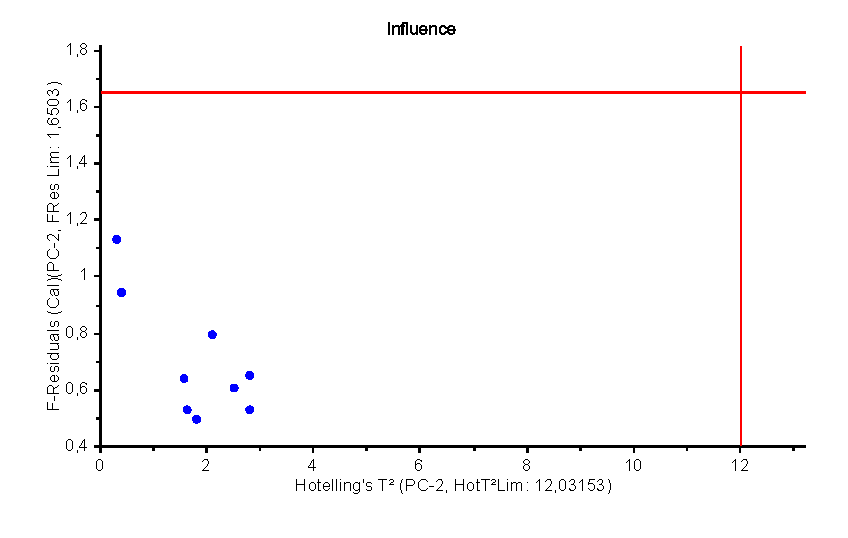
\includegraphics[width=\textwidth]{figurer/politikk-pca-influence}
 		\caption{}
 		\label{}
 	\end{subfigure}
 	\begin{subfigure}[t]{0.48\textwidth}
 		\centering
 		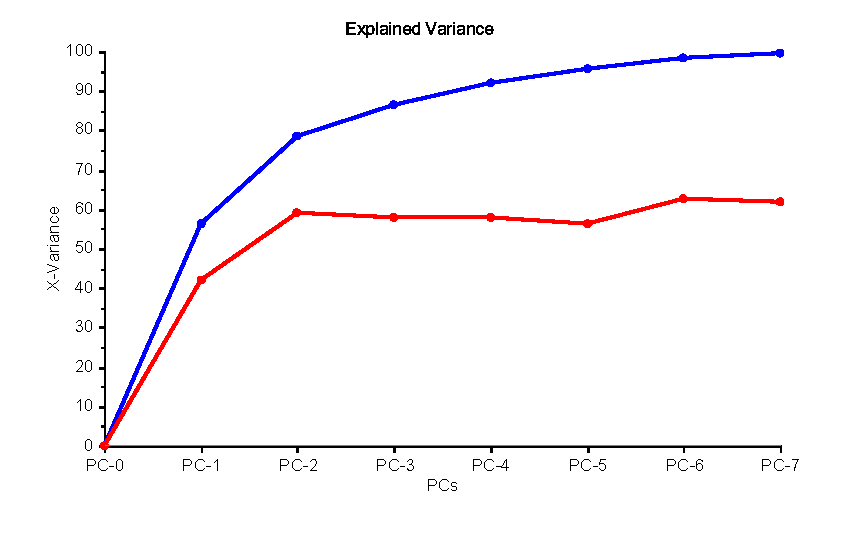
\includegraphics[width=\textwidth]{figurer/politikk-pca-ev}
 		\caption{}
 		\label{}
 	\end{subfigure}
	\label{fig:politikk-pca}
 \end{figure}
 

